% ============================================================
%  Toward Self-Correcting Glasses
%  Plain-language project proposal (rewritten for a non-optics reader)
%  Compile with: pdflatex main && bibtex main && pdflatex main (x2)
%  Upload PNGs from examples/output/ and checkpoints/ into a folder
%  called "figures" in your Overleaf project.
% ============================================================

\documentclass[11pt]{article}
\usepackage[margin=1in]{geometry}
\usepackage{graphicx}
\usepackage{hyperref}

\graphicspath{{figures/}}

\title{Toward Glasses That Test and Fix Your Eyes By Themselves}

\author{
  Mier Li \\
  Department of Computer Science \\
  University of North Carolina at Chapel Hill \\
  \texttt{mierli6566716@gmail.com}
}
\date{}

\begin{document}
\maketitle

\begin{abstract}
This project works toward a pair of glasses that can measure someone's eyeglass prescription by itself and physically adjust its own lenses to correct it, without an optometrist. Right now, that's still a research idea, not a finished product, so this document has two jobs: explain why the idea is worth pursuing and what's different about this particular approach, and then describe, in plain language and without the underlying optics mathematics, exactly what has been built and tested in software so far, why real hardware experiments are still needed even though the software works, and what the actual physical hardware plan looks like on the way to something wearable. No background in optics is assumed.
\end{abstract}

% ============================================================
\section{The problem, and why it's worth solving}
% ============================================================

Roughly 2.6 billion people worldwide need some kind of vision correction, and a large share of them don't have it \cite{who2019}. Uncorrected refractive error -- the technical name for needing glasses and not having them -- is the single most common cause of impaired vision on the planet. That's not because glasses are expensive or hard to manufacture. It's because getting a \emph{prescription} requires an eye exam, and an eye exam requires an optometrist: an appointment, travel, a wait, and in much of the world, a professional who simply isn't within reach. Even where access isn't a problem, it's still a recurring hassle -- prescriptions drift over time, especially in children whose eyes are still growing, so the whole process repeats every year or two indefinitely.

The motivating idea behind this project is a device that removes the professional from that loop entirely: glasses that look at your eye, work out your prescription on their own, and physically adjust their own lens power to correct it -- self-measuring, self-correcting, no optometrist required. That's an ambitious, multi-year hardware goal. This document is a snapshot of where things stand: what's already been proven in simulation, what real experiments are still needed and why, and what the actual path to physical hardware looks like.

% ============================================================
\section{What already exists, and what's actually different here}
\label{sec:existing}
% ============================================================

It helps to break "self-correcting glasses" into three separate problems, because each one, on its own, already has research behind it. Nobody has put all three together, and one of them is being approached here in a way that's meaningfully cheaper and simpler than the alternative already on the market.

\subsection{Measuring a prescription automatically}
There's a real, decades-old clinical technique called \emph{eccentric photorefraction} \cite{schaeffel1993, choi2000}. A small infrared light is placed just off to the side of a camera lens, a picture of someone's pupil is taken, and a bright crescent-shaped pattern shows up in that picture. The shape, size, and position of that crescent depends on the eye's prescription in a predictable, well-understood way -- no ``better or worse, one or two'' questions needed, unlike a normal eye exam. Devices that do this (autorefractors) already exist in clinics today. More recently, researchers have started training machine learning models to read that crescent pattern directly, instead of using hand-built formulas, with encouraging accuracy \cite{kim2025}.

\subsection{Changing a lens's power electronically}
Companies already sell lenses whose focusing power can be adjusted electrically, almost always using liquid crystal technology, similar to what's inside an LCD screen. The problem is cost and power draw: these tend to run on the order of \$1000 per lens at current production volumes, and they need a real voltage applied more or less continuously just to hold a setting -- not ideal for something meant to sit on someone's face all day, running off a small battery.

\subsection{Making blur disappear without touching the lens at all}
Separately, researchers at Berkeley and MIT showed that a displayed image can be pre-processed so that someone with blurry vision perceives it as sharp, with no corrective lens involved at all \cite{huang2014, pamplona2010}. It's a genuinely clever trick, but it only works for whatever is being shown on that specific screen -- it can't do anything about the rest of the room, or another person's face.

\subsection{So what's actually new here}
Nobody has connected the first two pieces into one working loop: sense the error automatically, and drive a correction automatically, using the same device. That integration -- not any single piece of it -- is the core contribution being pursued. The second thing that's different is a deliberate bet on \emph{how} to physically change a lens's power. Instead of liquid crystal, this project is built around a much older, much simpler mechanism called an Alvarez lens \cite{alvarez1967, barbero2011}, described in Section~\ref{sec:hardware}. In short: it's two oddly-curved pieces of plastic that sit in front of each other, and sliding them sideways by a small amount smoothly changes the focusing power. The design dates to 1967 and its patent expired decades ago, and the manufacturing process (molding curved plastic) is the same one already used to make ordinary sunglasses cheaply. It also doesn't need continuous power to hold a setting -- once it's slid into place, it just stays there mechanically. A rough cost estimate at real manufacturing volume comes out to single-digit dollars per lens, roughly two orders of magnitude below the liquid-crystal alternative.

% ============================================================
\section{What was actually built: a walk-through, start to finish}
% ============================================================

This section describes, step by step, everything that has been built and tested in software. None of it involves physical hardware yet -- that comes in Section~\ref{sec:hardware} -- but every step below is real, working code with measured results, not a sketch of a plan.

One clarification up front, because it matters for how to read this section correctly: the device being described here never gets to see the true answer. Every number quoted below as a ``true'' or ``known'' prescription exists only because this is a simulation, and simulations are written by people who obviously know what number they told the fake eye to have. That known number is used for exactly two things, and only two: generating realistic training examples ahead of time (Section~\ref{sec:cnn}), and grading how good a guess turned out to be, after the fact, purely so progress can be measured. The system itself, at the moment it's actually being used, only ever has access to a photograph -- never the answer key.

\subsection{Step 1 -- simulating what a blurry eye sees}
The starting point is a physics simulation that takes a prescription (the familiar sphere / cylinder / axis numbers printed on a glasses prescription) and computes what a person with that exact prescription actually sees when looking at something. The underlying method is the same branch of physics used to design telescope and camera optics: a perfect eye focuses a point of light down to essentially another point, but an eye with a refractive error smears that point into a small blob, and the shape and size of that blob depends on exactly how far off the prescription is. The simulation computes that blob directly from the prescription numbers, then applies it across an entire image to produce a realistic before-and-after of what that eye would see. Figure~\ref{fig:step1} shows several example prescriptions applied to the same test image -- notice how a simple near-sightedness (sphere-only) case blurs evenly in all directions, while adding astigmatism (cylinder) blurs more in one direction than another, matching what's clinically expected. This step is the physics engine that every later step depends on.

\begin{figure}[h]
  \centering
  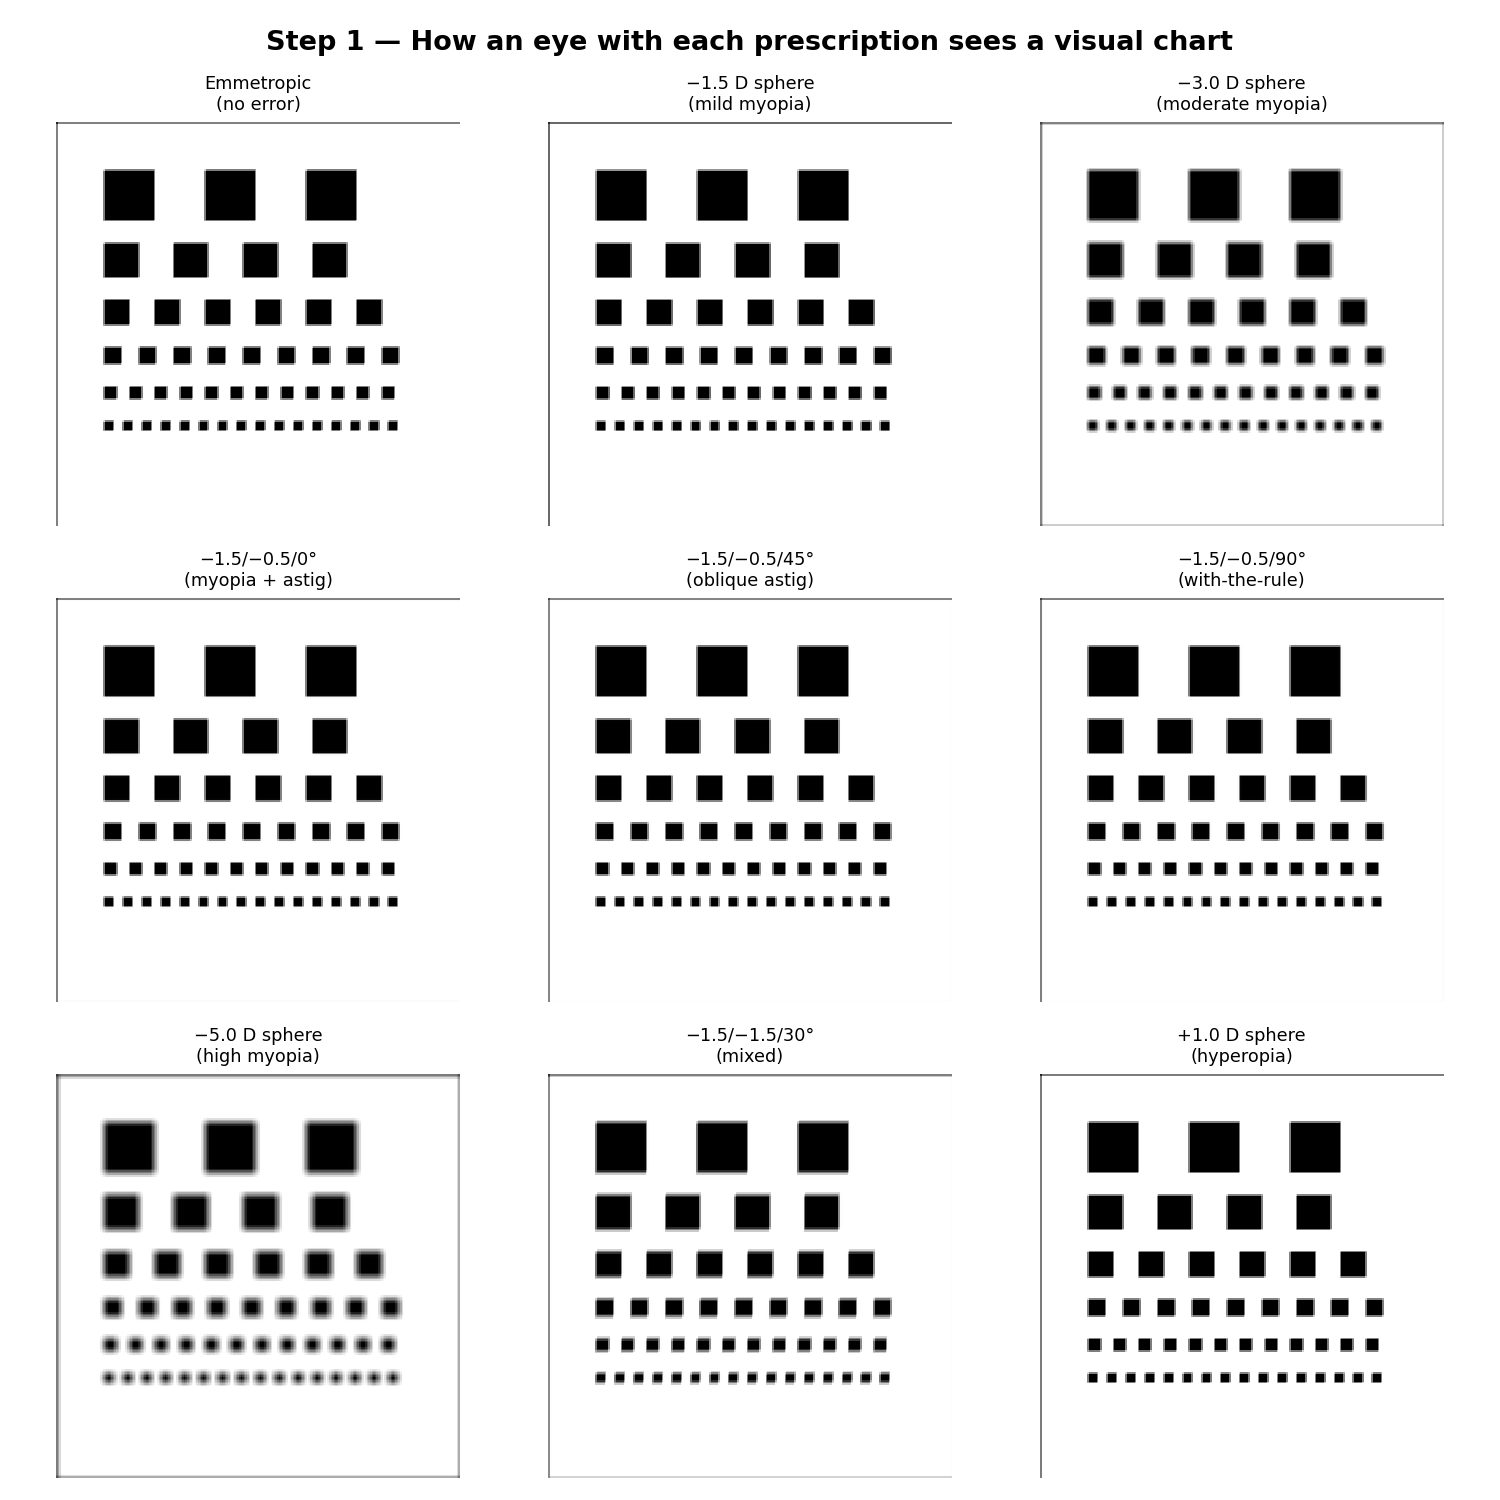
\includegraphics[width=\columnwidth]{step1_eye_blur.png}
  \caption{The same test chart as it would appear to nine different prescriptions, computed directly from the underlying optics.}
  \label{fig:step1}
\end{figure}

\subsection{Step 2 -- a working side demonstration: pre-distorting a screen}
As a standalone proof that the physics engine from Step 1 is correct and useful, it was applied in reverse: given a known prescription, an image can be deliberately pre-distorted so that, once blurred by that specific eye, it comes back into focus. Figure~\ref{fig:step2} shows this working end to end -- the pre-distorted image looks scrambled to a normal eye, but the target (blurry) eye perceives it as sharp. This doesn't require any new hardware at all; it only needs a display and a known prescription, and it's a genuinely complete, working result on its own, independent of the rest of this project.

\begin{figure}[h]
  \centering
  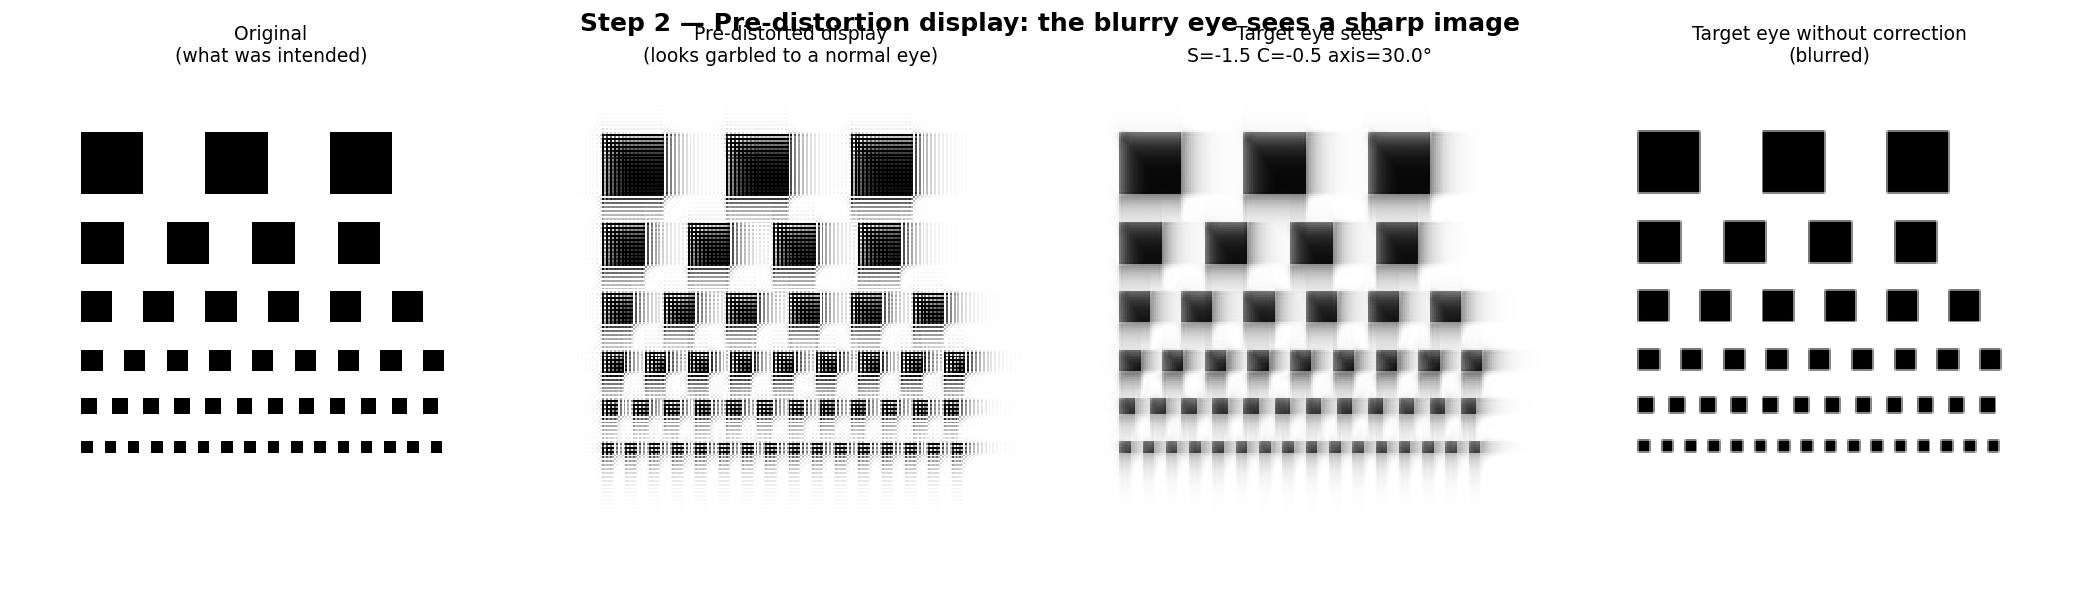
\includegraphics[width=\columnwidth]{step2_predistort.png}
  \caption{Left to right: the original image; the deliberately scrambled version sent to the screen; what a specific blurry eye actually perceives (sharp); what that same eye sees without any correction (blurry), for comparison.}
  \label{fig:step2}
\end{figure}

\subsection{Step 3 -- simulating the actual sensor: photorefraction images}
This is the step that matters most for the real device, because it's a simulation of the sensor that's actually planned for the hardware. Section~\ref{sec:existing} described eccentric photorefraction: an infrared light placed slightly off from a camera, photographing the pupil, producing a crescent-shaped pattern that depends on the eye's prescription. That entire physical process -- light entering the pupil, bouncing off the retina, and exiting at an angle that depends on the eye's focusing error -- was simulated directly from the same underlying optics as Step 1, producing realistic synthetic photographs of what that crescent would look like for any given prescription. Figure~\ref{fig:step4} shows a grid of these simulated crescent images across a range of prescriptions; notice how the crescent's position shifts as sphere power changes, and its shape changes with astigmatism. This is the raw material the next step learns from.

\begin{figure}[h]
  \centering
  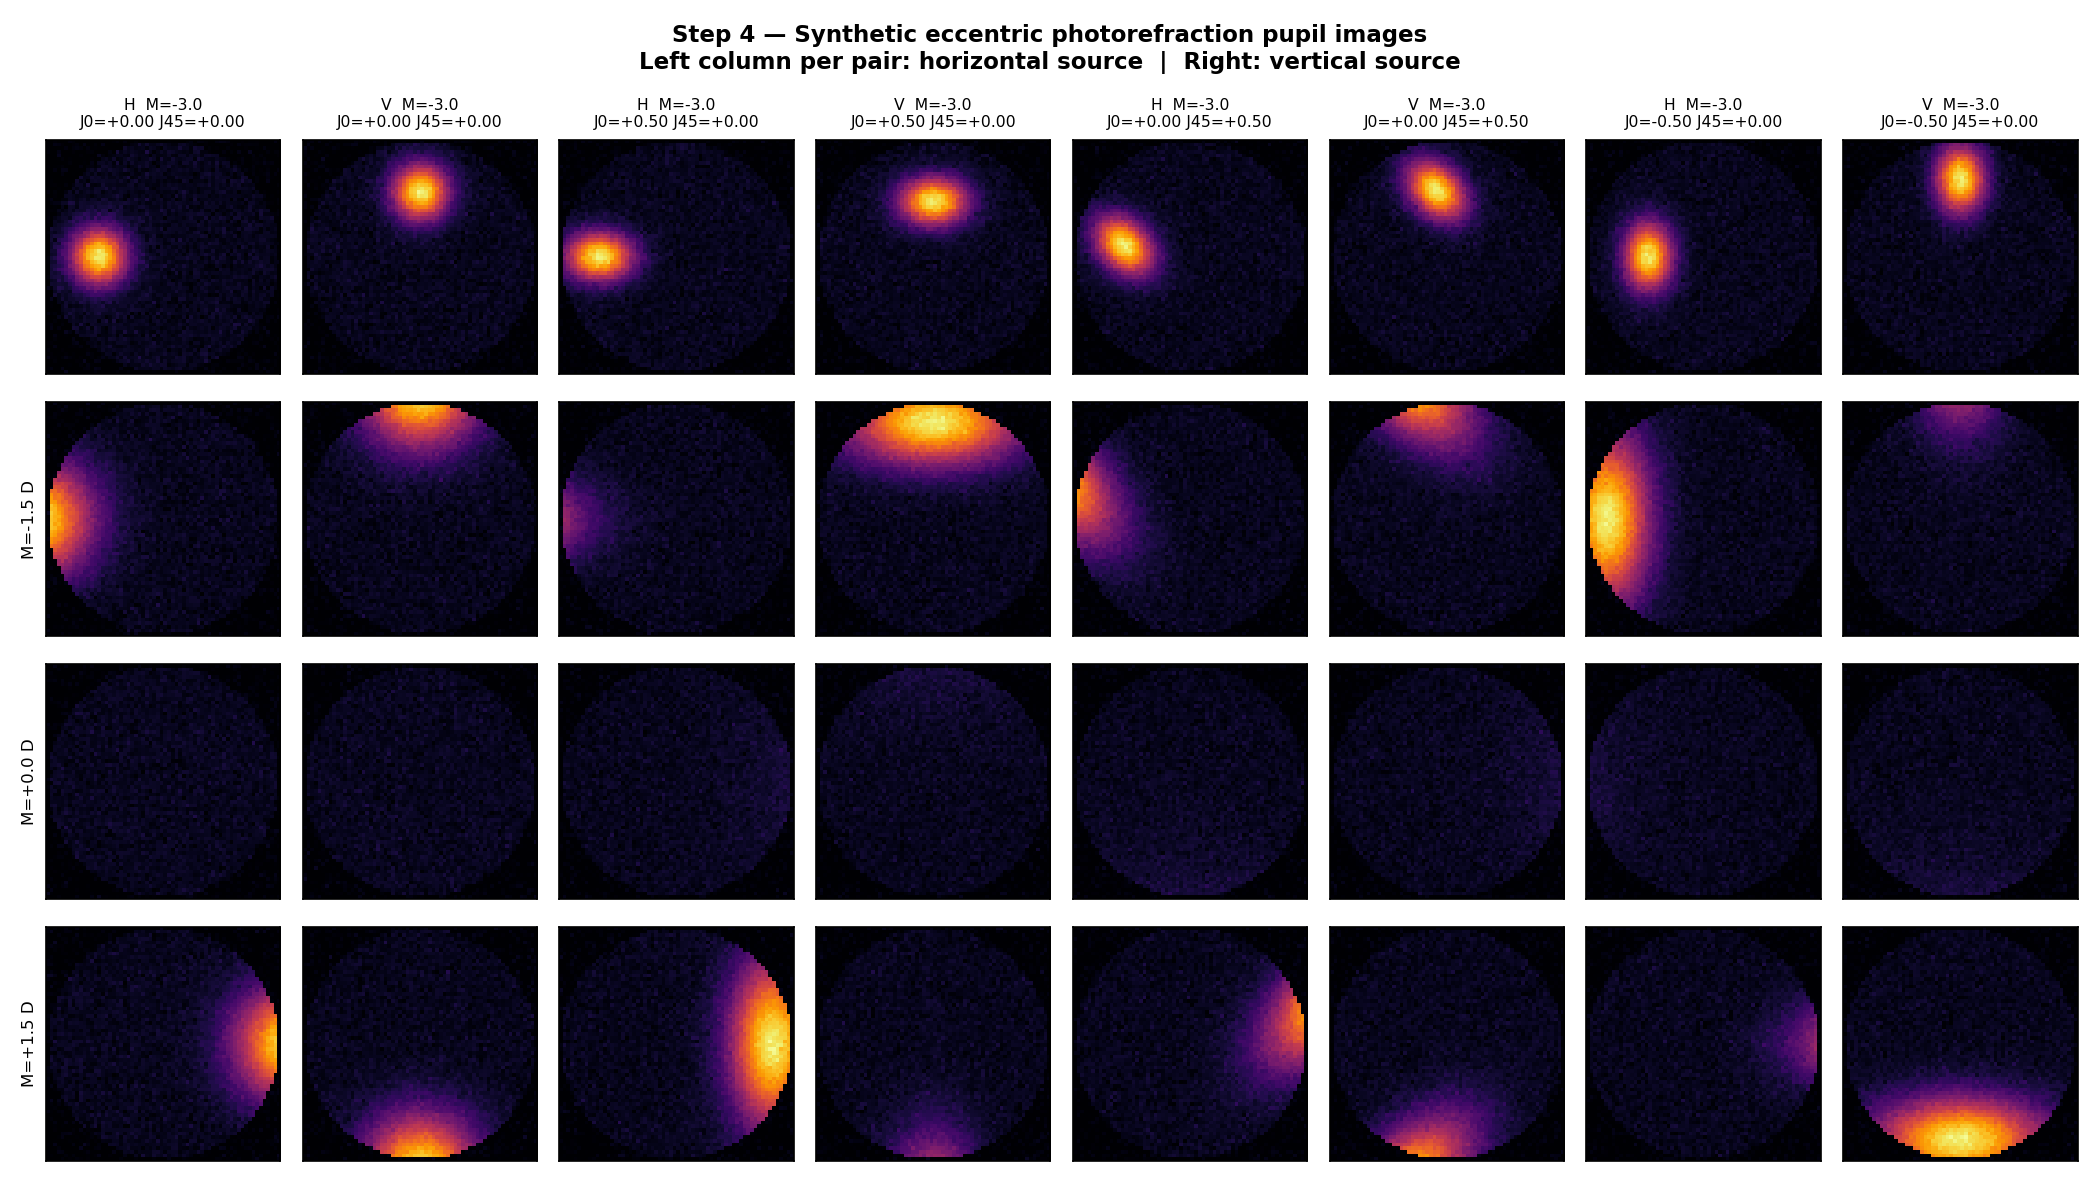
\includegraphics[width=\columnwidth]{step4_photorefraction.png}
  \caption{Simulated infrared pupil images across a range of prescriptions. Two images are produced per eye, from two slightly different light positions, because one light position alone can't fully separate all three prescription numbers.}
  \label{fig:step4}
\end{figure}

\subsection{Step 4 -- teaching a computer to read the crescent}
\label{sec:cnn}
A machine learning model (specifically, a small convolutional neural network, the same general kind of model used for ordinary image recognition) was trained to take one of these crescent images and output the three prescription numbers directly -- no manual formula, no iterative guessing, one photo in, one answer out. Roughly 100,000 simulated example crescents were generated for training, each with its known correct answer attached, and the model was trained to minimize the gap between its guess and that known answer, the standard way any supervised machine learning model is trained. Once training finished, the model was evaluated on 10,000 separate examples it had never seen during training, to get an honest measure of accuracy. It came out accurate to within roughly a quarter of a diopter (the standard unit prescriptions are measured in, and also the smallest step size an optometrist typically adjusts by) on two of the three prescription numbers, and somewhat less accurate, though still clinically meaningful, on the third -- Figure~\ref{fig:scatter} shows this directly, comparing the model's guesses against the true answers across the whole test set. A specific, well-understood cause was identified for why the third number is harder (Section~\ref{sec:limits}), which is exactly the kind of thing that's useful to know clearly before building physical hardware around it.

\begin{figure}[h]
  \centering
  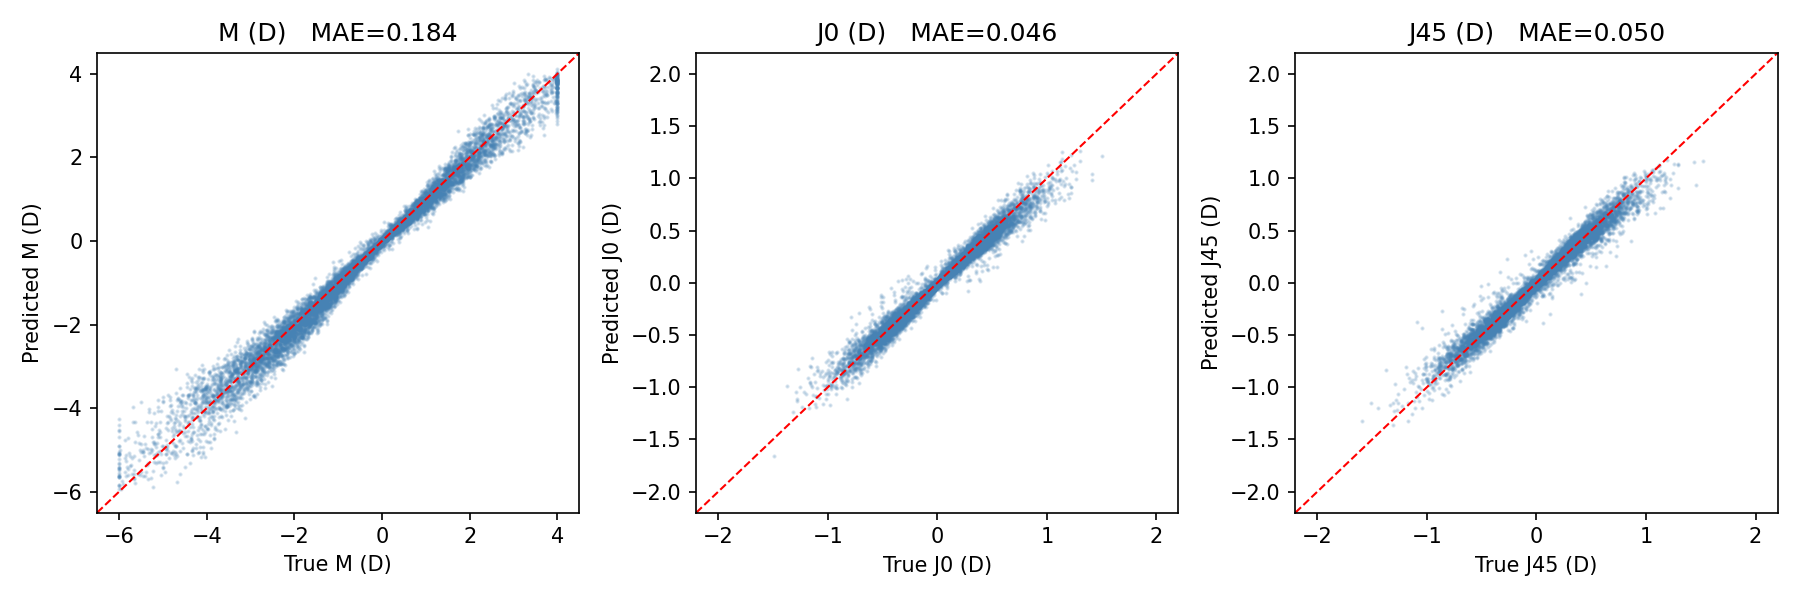
\includegraphics[width=\columnwidth]{test_scatter.png}
  \caption{Predicted vs.\ true values for each of the three prescription numbers, across 10,000 test examples the model never saw during training. A perfect model would place every point exactly on the diagonal line.}
  \label{fig:scatter}
\end{figure}

\subsection{Step 5 -- putting it together: sense, estimate, correct}
The final software step wires the previous ones into the actual device control flow a real pair of glasses would run: take a photo of the pupil (Step 3), feed it to the trained model (Step 4), and set the corrective lens to the exact opposite of whatever the model guessed. That's the whole loop -- one photo, one calculation, one lens adjustment, done. No back-and-forth, no trial and error, because none is needed: eccentric photorefraction is a direct, one-shot measurement, the same way a clinical autorefractor doesn't need to ask a patient any questions either. Figure~\ref{fig:storyboard} shows this complete sequence for one example eye, and across a batch of twenty randomly generated eyes, this one-shot correction alone brought the typical (median) residual error down from about 1.3 diopters uncorrected to about 0.08 diopters after correction -- comfortably inside the clinically meaningful range for essentially all of them.

\begin{figure}[h]
  \centering
  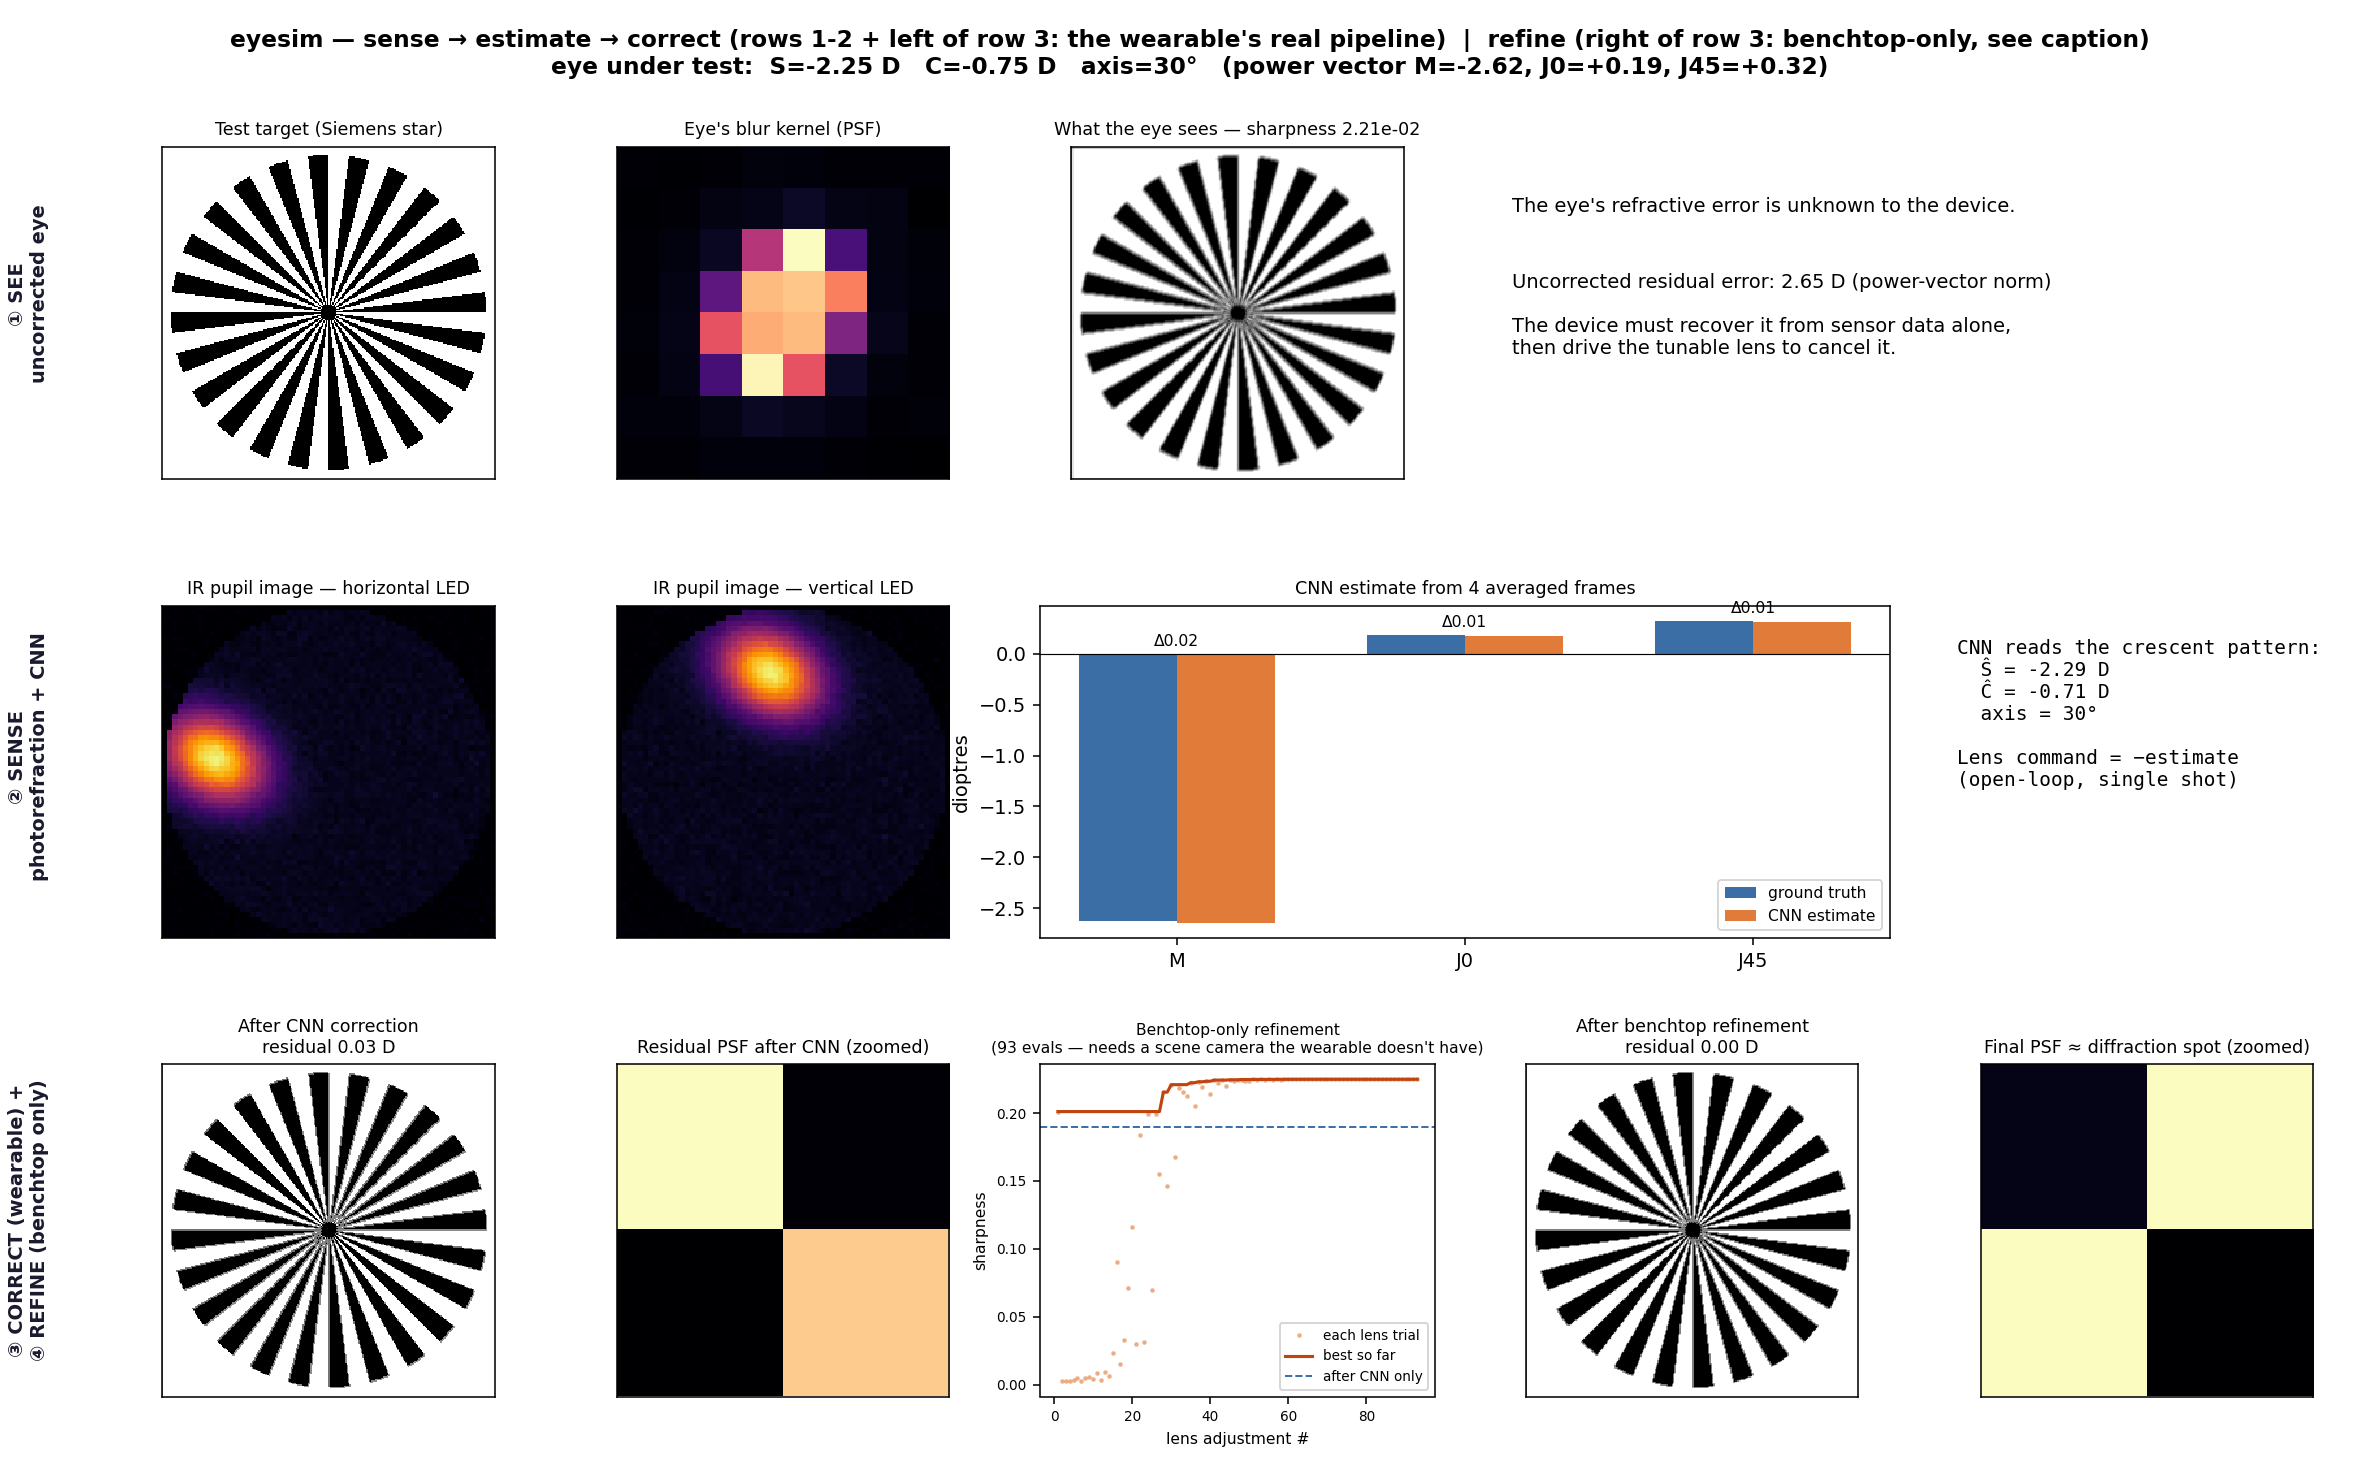
\includegraphics[width=\columnwidth]{pipeline_storyboard.png}
  \caption{The complete pipeline for one simulated eye: the uncorrected view, the two simulated sensor photos and the model's estimate compared to the true answer, and the corrected view. Everything left of the dashed line in the bottom row is what the real hardware is expected to be able to do; the panel to its right is a separate, optional capability discussed in Section~\ref{sec:hardware}.}
  \label{fig:storyboard}
\end{figure}

It's worth naming a strategy that was also explored in software but that turned out \emph{not} to match the real sensor being built, because working through why is genuinely informative. A second approach was tried where, instead of reading the answer from one photo, the system repeatedly adjusted the corrective lens while checking how sharp some test image looked -- essentially how a camera autofocuses. That idea works in general (autofocus is a real, everyday example of exactly this), but it needs a camera that can see roughly what the wearer's eye sees, looking outward at the world. The sensor actually being planned -- the pupil-facing infrared camera from Step 3 -- never looks at the world at all; it only ever photographs the wearer's own pupil, so it can never produce a ``how sharp does the world look right now'' measurement. That approach was set aside for the wearable device for exactly this reason, though it turns out to have a legitimate, different use described in Section~\ref{sec:hardware}.

\subsection{Being honest about current limits}
\label{sec:limits}
Two limitations are worth stating plainly, because they directly shape what hardware needs to prove next.

First, a specific, solvable ambiguity was found in the sensor simulation: the crescent pattern a camera would see depends on the true prescription \emph{and} on how far away the camera is from the eye, but only on the two multiplied together, not on either one separately. That means, in software alone, a stronger prescription measured from slightly farther away can look pixel-for-pixel identical to a milder prescription measured from slightly closer. In real hardware this is resolvable, because the physical camera-to-eye distance in a real pair of glasses is fixed and known by design, not a mystery -- but it explains precisely why one of the three prescription numbers is currently less accurate than the other two, and it's a concrete, well-defined problem to solve rather than a vague accuracy gap.

Second, and more generally: everything above was trained and tested entirely on simulated images, generated from a formula. A simulated photo, by construction, only ever looks exactly the way the underlying formula says it should. A real infrared camera photographing a real pupil will differ in ways a formula alone can't fully anticipate -- sensor noise, dust, stray reflections, imperfect alignment, and real human eyes having irregularities beyond the two kinds (near/far-sightedness and astigmatism) currently modeled. Closing that gap is precisely what Section~\ref{sec:hardware} is about.

% ============================================================
\section{Why real hardware is still needed, and what it actually means}
\label{sec:hardware}
% ============================================================

Given that the software above already works, it's fair to ask why physical hardware is necessary at all before this could be trusted. The honest answer is that a simulation can only ever be as good as the assumptions built into it, and some things genuinely cannot be discovered except by building something real and testing it.

\subsection{A physical stand-in for an eye, with a known, adjustable prescription}
The single most important piece of hardware needed next is not a finished wearable device -- it's a benchtop rig that can stand in for a human eye with a prescription that can be dialed to any exact, known value on demand. The idea is to build a fixed lens representing the eye's optics, paired with a small, precisely adjustable slider that moves a light-scattering surface (standing in for the retina) back and forth. Moving that slider by a known amount corresponds to a known, calculable shift in prescription -- the same optics from Section~\ref{sec:existing} apply directly, just running in reverse. A rotating cylindrical lens in front handles astigmatism, at any axis. The result is a physical object that can be set to any prescription the software can simulate, then photographed for real with a real infrared camera and light, producing a real photo with a known, trustworthy correct answer attached.

This solves two separate problems at once. First, it directly tests whether the trained model (Section~\ref{sec:cnn}) still works on a real photograph, not just a simulated one -- and if it doesn't work as well, the resulting real, labeled photos are exactly what's needed to retrain and improve it, closing the sim-to-real gap named in Section~\ref{sec:limits} with real evidence instead of guesswork. Second, because this rig involves an actual camera photographing an actual test pattern through actual optics, it's exactly the situation where the sharpness-based strategy set aside in Section~\ref{sec:hardware}'s predecessor becomes useful again: it can be used to double-check the rig's own mechanical calibration (does sliding the retina by a measured amount actually shift the effective prescription by the predicted amount?) and, separately, to confirm that a sharpness-searching control algorithm converges reliably against real camera noise, independent of whether the trained model exists at all.

\subsection{What else can only be learned from real hardware}
A few other things fall into the same category -- not fixable in software, only discoverable by building something:
\begin{itemize}
  \item \textbf{Does the corrective lens behave as predicted?} The Alvarez lens described in Section~\ref{sec:innovation} needs to be physically built and measured: does sliding it by a given distance really change its focusing power by the amount the underlying formula predicts?
  \item \textbf{Does the whole system work fast enough and use little enough power?} A real onboard camera, chip, and small motor all draw real power and take real time to run; whether the correction feels effectively instant, and whether battery life is reasonable for something worn all day, can only be measured on real hardware.
  \item \textbf{Does it still work in normal lighting?} Sunlight itself is a strong source of infrared light, and a real environment needs to be tested to see whether that interferes with the sensor.
  \item \textbf{Real eyes are messier than simulated ones.} Eventually, with proper research oversight and informed consent, testing needs to move to real human eyes and be compared against a real clinical reference (an actual autorefractor or optometrist). Real eyes blink, move, change pupil size with lighting, and have optical quirks beyond the two kinds currently modeled -- none of which show up in a simulated eye no matter how carefully it's built.
\end{itemize}

% ============================================================
\section{The corrective lens, and the path to actual glasses}
\label{sec:innovation}
% ============================================================

The sensing side of this project (Sections~\ref{sec:cnn}--\ref{sec:hardware}) answers ``what is this person's prescription.'' A separate piece is needed to physically act on that answer: something that changes a lens's focusing power on command, cheaply enough and with little enough power draw to actually live inside a pair of glasses. As described in Section~\ref{sec:existing}, the mainstream option (liquid crystal lenses) is roughly a thousand dollars per lens and needs continuous voltage to hold a setting -- both serious obstacles for a wearable, battery-powered, mass-producible device.

The alternative being pursued instead is the Alvarez lens, patented in 1967 and now in the public domain \cite{alvarez1967, barbero2011}. The core idea is genuinely simple: two identically-shaped, unusually-curved pieces of plastic are placed directly in front of each other. On their own, each piece barely does anything optically. But sliding them sideways relative to each other, by a distance of well under a millimeter, smoothly changes the combined focusing power of the pair -- more slide, more power, in a precisely predictable relationship. Two such pairs per eye, one oriented normally and one rotated forty-five degrees, together provide enough control to correct any combination of the three prescription numbers this project measures. Because the mechanism is purely mechanical, it holds its position with no power at all once set, unlike liquid crystal, and because the curved-plastic shape is exactly the kind of part that can be inexpensively injection-molded at scale (the same manufacturing process used for ordinary sunglasses lenses), a rough cost estimate at production volume comes out to single-digit dollars per lens.

\subsection{From here to a wearable device}
Putting everything above in order, the realistic path from where this project currently stands to an actual pair of self-correcting glasses looks like this:

\begin{enumerate}
  \item \textbf{Build the model-eye bench rig} (Section~\ref{sec:hardware}) -- this is the immediate next step, and it does double duty: generating real labeled training photos, and providing a testbed to validate the control algorithms already written.
  \item \textbf{Build and measure the Alvarez lens on its own bench}, separately from the sensing side, confirming that its real focusing power matches the predicted relationship to slide distance.
  \item \textbf{Combine both benches into one working loop}: a real photorefraction camera reading a real or model eye, a model retrained on real photos estimating the prescription, and that estimate driving the real Alvarez lens automatically. This is the first point where the entire loop runs for real, even though it's still a bulky lab setup rather than something wearable.
  \item \textbf{Miniaturize} the camera, onboard processing, actuator, and battery to fit inside an actual glasses frame.
  \item \textbf{Validate against real human eyes} and a real clinical reference, under appropriate research oversight, and iterate based on how far off the device's readings are from ground truth.
  \item \textbf{A genuinely wearable, all-day product} is the final step, deliberately last, since it's the highest bar and realistically well beyond the scope of a single project phase on its own. Each step before it is independently useful and demonstrable, which matters, since the last step is likely to take considerably longer than everything before it combined.
\end{enumerate}

% ============================================================
\section{Conclusion}
% ============================================================

The software described here is a complete, working, measured simulation of an autonomous refraction device: a physics engine that turns a prescription into realistic blur, a working demonstration that the same physics can pre-correct a screen image, a simulated sensor that produces realistic photorefraction images, a trained model that reads a prescription directly from one such image with clinically meaningful accuracy, and a full pipeline that wires sensing, estimation, and correction into the same one-shot control flow a real device would use. What it cannot yet answer is whether any of this survives contact with a real camera, a real lens, and a real eye -- which is exactly what the next phase of hardware work, starting with the model-eye bench rig, is designed to find out.

\bibliographystyle{plain}
\bibliography{refs}

\end{document}
